\subsection{Examples}

\begin{frame}
	\begin{block}{Car Evaluation Dataset}
		\begin{itemize}
			\item Buying price (B): v-high, high, med, low
			\item Maintain cost (M): v-high, high, med, low
			\item Doors (D): two, three, four, more
			\item Persons (P): two, four, more
			\item Luggage boot (L): small, medium, big
			\item Safety (S): low, medium, high
		\end{itemize}
	\end{block}
	%Using First-order Logic we have:
	%\begin{block}{}
	%	\begin{itemize}
	%		\item $\forall c, {Buying}( c , high ) \rightarrow {Doors}( c , four ) \land {Persons}( c , more )$
	%		\item $\forall c, {Maintain}( c , low ) \rightarrow {Safety}( c , high )$
	%	\end{itemize}
	%\end{block}
	%But, how to represent:
	Represent:
	\begin{block}{}
		\begin{itemize}
			\item Half of cars that have four doors have a medium luggage boot
			\item 15\% of cars are low safety, 77\% medium safety and 8\% high safety
		\end{itemize}
	\end{block}
\end{frame}
	
\begin{frame}
	Using a probabilistic model of knowledge to represent all possible relations we have:
	\begin{block}{}
		\[ \P( B , M , D , P , L , S ) \]
	\end{block}
	This requires $4 \times 4 \times 4 \times 3 \times 3 \times 3 = 1728$ probabilities hard to estimate, but we can drastically reduce this number by assuming (conditional) independences
\end{frame}
	
\begin{frame}[fragile]
	For example:
	\begin{figure}
		\centering
		\begin{tikzpicture}[ scale = 0.6 ]
	\tikzset{ vertex/.style = { shape = rectangle , draw , minimum size = 2em , rounded corners } }
	\tikzset{ edge/.style = { ->,> = latex' } }
	% vertices
	\node[ vertex ] (B) at  ( 4 , 4 ) { ${Buying}$ } ;
	\node[ vertex ] (D) at  ( 2 , 2 ) { ${Doors}$ } ;
	\node[ vertex ] (P) at  ( 6 , 2 ) { ${Persons}$ } ;
	\node[ vertex ] (M) at  ( 0 , 0 ) { ${Mantain}$ } ;
	\node[ vertex ] (S) at  ( 4 , 0 ) { ${Safety}$ } ;
	\node[ vertex ] (L) at  ( 8 , 0 ) { ${Luggage}$ } ;

	%edges
	\draw[ edge ] (B) to (D) ;
	\draw[ edge ] (B) to (P) ;
	\draw[ edge ] (D) to (M) ;
	\draw[ edge ] (D) to (S) ;
	\draw[ edge ] (P) to (S) ;
	\draw[ edge ] (P) to (L) ;
\end{tikzpicture}
	\end{figure}
	\begin{block}{}
		\begin{itemize}
			\item \alert{Doors} and \alert{Persons} are independent given \alert{Buying}: $\P( D , P \mid B ) = \P( D \mid B ) \P( P \mid B )$
			\item \alert{Mantain} and \alert{Safety} are independent given \alert{Doors}: $\P( M , S \mid D ) = \P( M \mid D ) \P( S \mid D )$
			\\$\vdots$
		\end{itemize}
	\end{block}
\end{frame}

\begin{frame}[fragile]
	\begin{figure}
		\centering
		\begin{tikzpicture}[ scale = 0.6 ]
	\tikzset{ vertex/.style = { shape = rectangle , draw , minimum size = 2em , rounded corners } }
	\tikzset{ edge/.style = { ->,> = latex' } }
	% vertices
	\node[ vertex ] (B) at  ( 4 , 4 ) { ${Buying}$ } ;
	\node[ vertex ] (D) at  ( 2 , 2 ) { ${Doors}$ } ;
	\node[ vertex ] (P) at  ( 6 , 2 ) { ${Persons}$ } ;
	\node[ vertex ] (M) at  ( 0 , 0 ) { ${Mantain}$ } ;
	\node[ vertex ] (S) at  ( 4 , 0 ) { ${Safety}$ } ;
	\node[ vertex ] (L) at  ( 8 , 0 ) { ${Luggage}$ } ;

	%edges
	\draw[ edge ] (B) to (D) ;
	\draw[ edge ] (B) to (P) ;
	\draw[ edge ] (D) to (M) ;
	\draw[ edge ] (D) to (S) ;
	\draw[ edge ] (P) to (S) ;
	\draw[ edge ] (P) to (L) ;
\end{tikzpicture}
	\end{figure}
	\begin{block}{}
		$\P( B , M , D , P , L , S ) = \P( B ) \P( D \mid B ) \P( P \mid B ) \P( M \mid D ) \P( S \mid D , P ) \P( L \mid P )$
	\end{block}
	This requires $4 + (4 \times 4) + (3 \times 4) + (4 \times 4) + (3 \times 4 \times 3) + (3 \times 3) = 93$ probabilities instead of $1728$
\end{frame}
	
\begin{frame}[fragile]
	\begin{columns}
		\begin{column}{.3\linewidth}
			Consider each variable has $k$ values:\\
			We requires $k^{33}$ probabilities without independences.
		\end{column}
		\begin{column}{.6\linewidth}
			\begin{figure}
				\centering
				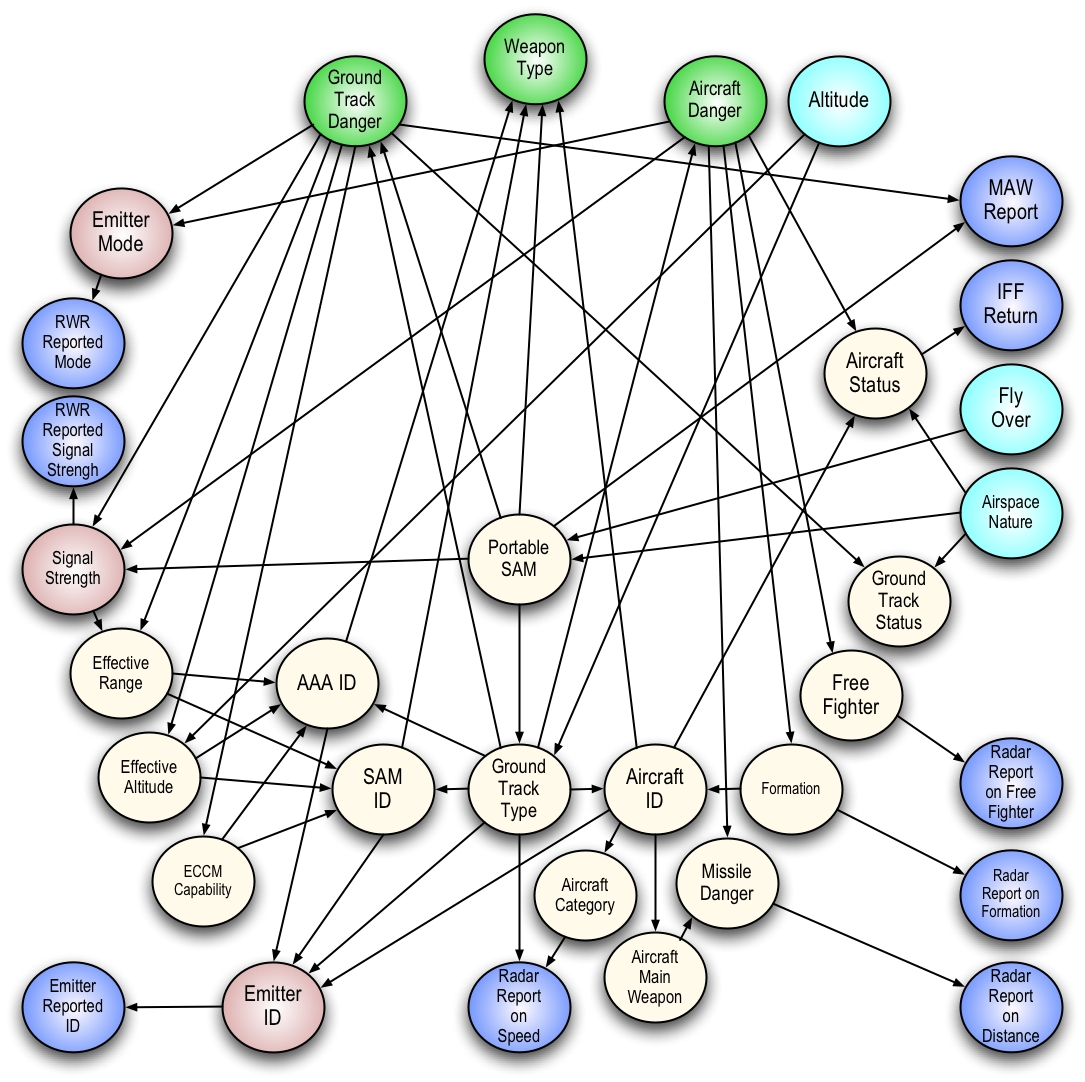
\includegraphics[height=17em]{images/complexbn}
			\end{figure}
		\end{column}
	\end{columns}
\end{frame}